\documentclass[11pt]{article}

\usepackage{latexsym}
\usepackage{amsmath}
\usepackage{amssymb}
\usepackage{amsthm}
\usepackage{graphicx}
\usepackage{float}
\usepackage{wrapfig}
\usepackage{pseudocode}
\usepackage{url}
\usepackage[backref, colorlinks=true, citecolor=red, urlcolor=blue, pdfauthor={Jyh-Ming Lien}]{hyperref}
\graphicspath{{images/}}

\newcommand{\handout}[5]{
  \noindent
  \begin{center}
  \framebox{
    \vbox{
      \hbox to 5.78in { {\bf } \hfill #2 }
      \vspace{4mm}
      \hbox to 5.78in { {\Large \hfill #5  \hfill} }
      \vspace{2mm}
      \hbox to 5.78in { {\em #3 \hfill #4} }
    }
  }
  \end{center}
  \vspace*{4mm}
}

\newcommand{\lecture}[4]{\handout{#1}{#2}{#3}{#4}{#1}}

\newtheorem{theorem}{Theorem}
\newtheorem{corollary}[theorem]{Corollary}
\newtheorem{lemma}[theorem]{Lemma}
\newtheorem{observation}[theorem]{Observation}
\newtheorem{proposition}[theorem]{Proposition}
\newtheorem{definition}[theorem]{Definition}
\newtheorem{claim}[theorem]{Claim}
\newtheorem{fact}[theorem]{Fact}
\newtheorem{assumption}[theorem]{Assumption}

% 1-inch margins, from fullpage.sty by H.Partl, Version 2, Dec. 15, 1988.
\topmargin 0pt
\advance \topmargin by -\headheight
\advance \topmargin by -\headsep
\textheight 8.9in
\oddsidemargin 0pt
\evensidemargin \oddsidemargin
\marginparwidth 0.5in
\textwidth 6.5in

\parindent 0in
\parskip 1.5ex
%\renewcommand{\baselinestretch}{1.25}

\begin{document}

\lecture{Voronoi Stippling Report}{Fall 2017}{Anthony Sermania}{Computational Geometry}

\section{Summary of the two methods}

\subsection{hedcuter method}
The hedcuter method is as follows:

Hedcut:
\begin{enumerate}
\item Create a set of n random initial points (keep on random probability, favoring darker areas)
\item Compute the Weighted Centroidal Voronoi Tessellation (CVT)
\item Generate Disks
\end{enumerate}

Computing The CVT:
\begin{enumerate}
	\item While (we have fewer iterations than the limit AND the max-displacement is greater than some threshold:
	\begin{enumerate}
	\item Computer the Voronoi
	\item Shift Voronoi cell sites towards cell centroids (and record displacement
	\end{enumerate}
\end{enumerate}


Compute the Voronoi
\begin{enumerate}
\item For each input site
	\begin{enumerate}
	\item redirect site to corresponding position in resized image (fake enhanced resolution)
	\item determine distance based on color of site
	\item add site to open list/heap
	\end{enumerate}
	
\item while heap is not empty
\begin{enumerate}
	\item cell <- max heap element (pop)
	\item if distance has been updated or cell has been visited
		\begin{enumerate}
		\item skip
		\end{enumerate}
		
	\item for each neighbor of cell
	\begin{enumerate}
	\item if cell.distance+neighbor.distance < neighbor.distance
	\begin{enumerate}
	\item set neighbor.distance <- cell.distance+neighbor.distance
			\item make neighbor.root <- cell.root
			\item push neighbor into heap
	\end{enumerate}
			
	\end{enumerate}
		
\end{enumerate}
	
\item For each cell in image
	\begin{enumerate}
	\item determine root of cell
	\item add cell to cell.root's coverage
	\end{enumerate}
	
\item Remove all cells with coverage.empty
\end{enumerate}


Move voronoi cell sites to their new locations (and record displacement)
\begin{enumerate}
\item For each cell
\begin{enumerate}
\item calculate new position as average of positions in coverage
\item Generate high res img
\item newpos <- (0, 0), total <- 0
\item for each cell c in cell.coverage
\begin{enumerate}
\item newpos += c.distance*c.pos
\item total += c.distance
\end{enumerate}

\item newpos /= total to normalize
\item newpos /= subpixels to redirect to original image
\item store manhattan distance from new to old position
\end{enumerate}

\item return the max displacement (manhattan distance) or average of displacements (depending on termination mode)
\end{enumerate}


Generate Disks
\begin{enumerate}
\item Collect the darkness/color of the area in a voronoi cell
\item Create a disk at cell site (center)
\item Color/darken cell according to the average color/darkness of the pixels i the cell
\end{enumerate}


\subsection{voronoi method}
This one was a little bit tougher to work through mentally. At the highest level it uses Lloyd's Algorithm as so:

While generating points (xi) not converged to centroid
\begin{enumerate}
\item compute voronoi diagram of xi
\item compute centroid Ci
\item move generating point xi to centroid Ci
\end{enumerate}


The Voronoi diagram computation is done differently here, utilizing an entire Voronoi Generation class that appears to implement a half-edge mechanism for doing it's work after some initial set up. It is extremely well commented; rather than just essentially replicating the comments, here is an overview of the half-edge voronoi generation:

\begin{enumerate}
\item While there are events:
\begin{enumerate}
\item If the lowest site is lower than the lowest vector intersection process the site
\begin{enumerate}
\item Get left and right half edges, plus the edge of the left halfedge (or the bottom site if there's no edge)
\item create a bisector for the left edge (or bottom site) and if it intersects the left edge shuffle the vertices so the left edge and bisector share a vertex.
\item Create a new half edge right of the first (only at the moment) bisector
\item if this new bisector intersects with the right halfedge, add the bisector halfedge to the ordered linked list of verts
\item get next site
\end{enumerate}

\item else process the lowest vector intersection
\begin{enumerate}
\item Get the halfedge for the intersection vector, as well as the surrounding halfedges
\item get the sites of the of the exterior halfedges
\item consider a circle passing through the triple of sites obtained
\item get the vertex that caused the event
\item set the endpoints of the left and right half edges to be this vertex
\item mark the lowest half edge for deletion
\item clear events for right halfedge
\item mark right halfedge for deletion
\item if the site to left of the event is higher than site to the right, swap them
\item create an edge between the two sites
\item create a half edge for this edge
\item insert the new bisector to the right of the left halfedge
\item cleanup (reposition half-edges not intersecting the bisector that should)
\end{enumerate}

\end{enumerate}

\end{enumerate}


That still got pretty verbose, but it's not quite done. Once this routine has run, the generator that ran it is used to collect the edges before completing (this process is straightforward and is not detailed here).

Now it moves to step 2, redistributing the stipples (bringing them closer to the centroids of the Voronoi cells). This is done in parallel where applicable.

\begin{enumerate}
\item Do some setup (make pairs of points and edge lists)
\item For each pair:
\begin{enumerate}
\item Calculate Centroid
\item update Radius and vertex X/Y positions to be that of the calculated centroid
\item determine displacement of point
\end{enumerate}
\item average displacement of all points
\end{enumerate}


Calculating a Centroid:
According to the paper, \textit{Weighted Voronoi Stippling} by Adrian Secord, there are some integrals being done here. The implementation provided however seems to work around that, operating primarily on distance constraints:

\begin{enumerate}
\item Compute the Clip Lines
\item For all points in this space if a point is inside it's polygon, it contributes to the area density
\item If a cell is not completely white, shift the centroid according to the weighted-spot:area density ratio (that's a weird way to put it, but it's what's happening)
\item Iterate over the available edges and determine the nearest and farthest, using one of those distances to determine the size of the stipple (nearest if NoOverlap, Farthest otherwise) and scale by the area:max-area ratio
\item Return the pair of the original point and the radius.
\end{enumerate}



\section{Comparison of the two methods}
Both methods saw fair success. I will however claim the voronoi code to be superior overall.

Let's start with hedcut though. For one thing, hedcut was not consistent across multiple runs with the same parameters. Take for instance the following images:

\begin{figure}[H]
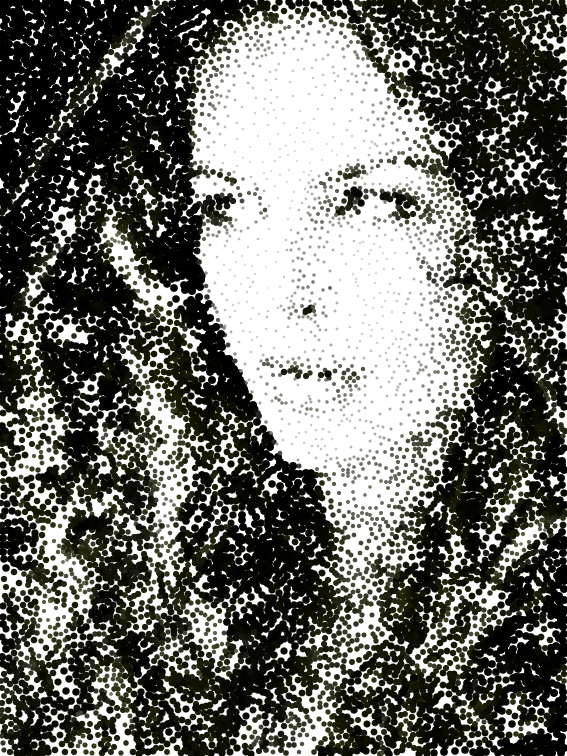
\includegraphics[scale=0.4]{fairyeyes-10000-r4-1.png}
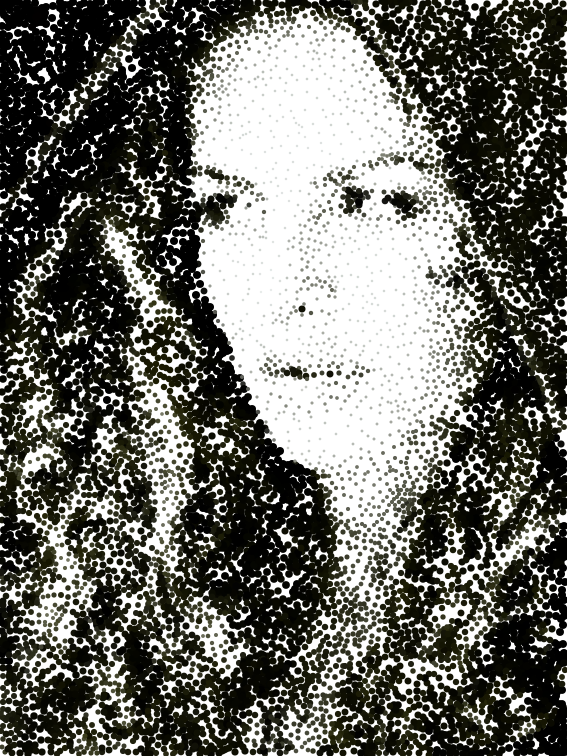
\includegraphics[scale=0.4]{fairyeyes-10000-r4-2.png}
\end{figure}

We can see here that the two images, run with the same parameters (radius 4, 10,000 stipples) produced different stipplings. By contrast, here are two images from the voronoi code with the equivalent parameters (4,000 stipples, color, overlap)

\begin{figure}[H]
\includegraphics[scale=0.4]{fairyeyes-4k-color-2.png}
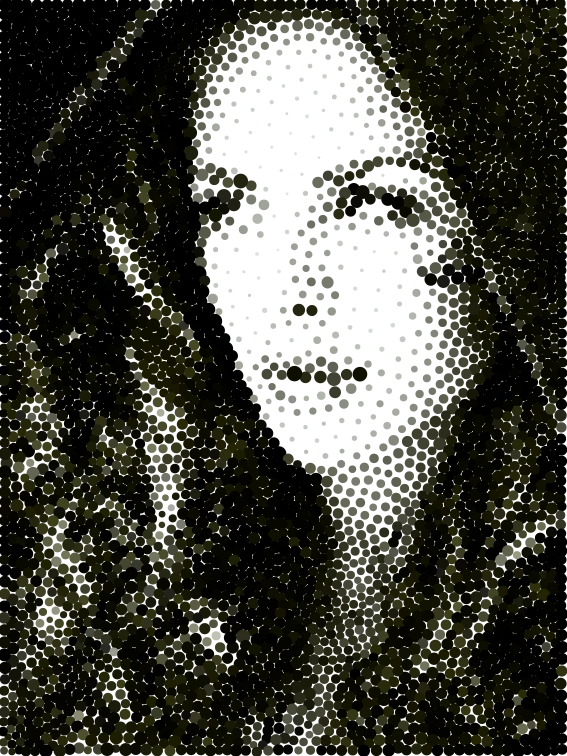
\includegraphics[scale=0.4]{fairyeyes-4k-color-3.png}
\end{figure}

And two more from voronoi, this time with no overlap.

\begin{figure}[H]
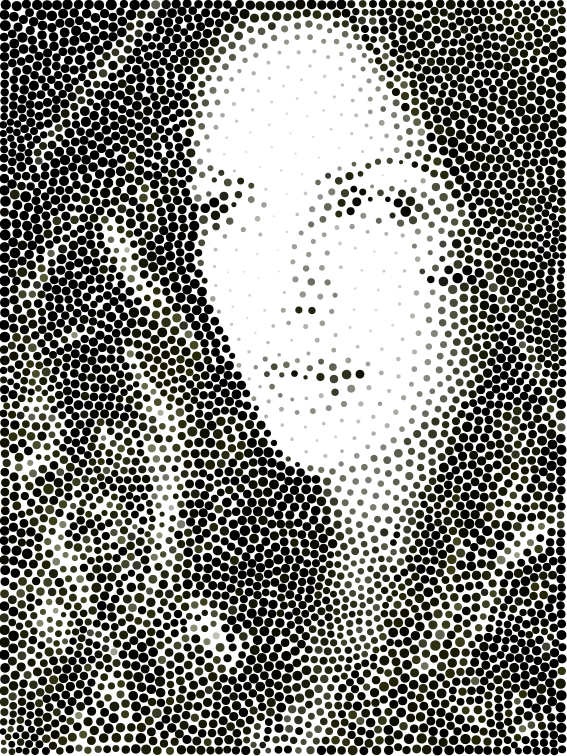
\includegraphics[scale=0.4]{fairyeyes-noverlap-4k-color.png}
\includegraphics[scale=0.4]{fairyeyes-noverlap-4k-color-2.png}
\end{figure}

It is worth noting I discovered later that hedcut might by consistent with sufficiently many iterations (see Improvements).

In terms of speed, hedcut may be faster in the simplest circumstances, coming out at around the same computatin time for 10,000 stipples as voronoi did for 4,000 and 8,000, however voronoi never seemed to vary much with number of dots- just by image. Hedcut on the other hand does take longer the more dots there are. The two images below are both 100,000 stipples. The image on the left is the hedcut image, created in 16.22 seconds; the one on the right is from voronoi, created in 4.43 seconds (not substantially slower than the 8,000 or 4,000 stipple runs for voronoi).

\begin{figure}[H]
\includegraphics[scale=0.4]{fairyeyes-hedcut-100000.png}
\includegraphics[scale=0.4]{fairyeyes-voronoi-100000.png}
\end{figure}

Beyond that time difference, the level of image fidelity with this many stipples is vastly superior in the voronoi image. I suspect the difference in speed comes from the use of so many loops in the hedcut code. The difference in quality is undoubtedly due to the stronger implementation of varied stipple sizes (based purely on the voronoi cell size) in the voronoi code. The hedcut code uses a base radius which is scaled, resulting in much weirder stipple sizes. It does however improve it's image fidelity with successive iterations (see below), perhaps even gaining on voronoi for image quality.

\section{Improvement of hedcuter method}
While I technically made two improvements to hedcut, I can only claim one of them was significant. The insignificant one was some compiler optimizations; this ended up not amounting to any consistently measurable improvement, and moreover wasn't a significant revamp to the code, so I would understand considering it poorly. Given that I was working on Windows in the end, and this required some working knowledge of Visual Studio (2013), maybe it's worth something? I ultimately did not try a third attempt due to time- much of which was wasted either trying to get the project to run (copy-paste .dll saved the day) or interviewing CS 110 students one at a time.

I did however make one very significant change that yielded marvelous improvements. There was a point in move-sites where the code was creating a higher resolution version of our source image to do centroid-relocation math in before redirecting the result back to the source image resolution. Being located in move-sites, it was being run for every voronoi cell, every iteration of the algorithm. This struck me as highly inefficient. So I relocated it to just before we began running the algorithm in full- we never change the source image, so the higher res version should never change either. I was initially confused because I was mistakenly attributing the benefits of greater iterations to this change, but I did discover my folly.

\begin{figure}[H]
\includegraphics[scale=0.5]{sunbros-plain-itr1-100000.png}
\includegraphics[scale=0.5]{sunbros-plain-itr3-100000.png}
\caption{Original Code. Left is 1 iteration; Right is 3 iterations. A fair improvement can be seen by increasing the number of iterations.}
\end{figure}

\begin{figure}[H]
\includegraphics[scale=0.5]{sunbros-lessrescale-itr1-100000.png}
\includegraphics[scale=0.5]{sunbros-lessrescale-itr3-100000.png}
\caption{The revised version. As before, left is 1 iteration and right is 3. The images are quite similar to their original counterparts. It is possible the hedcut algorithm gains consistency with increasing iterations- a costly but evidently worthwhile gain.}
\end{figure}

So, No significant changes in the images from this. However, consider for a moment the following tables, indicating run times for various runs using the sunbros.png image for 1 or 3 iterations, before and after the change.

\begin{figure}[H]
\includegraphics[scale=0.8]{hedcut-table.png}
\end{figure}
\begin{figure}[H]
\includegraphics[scale=0.8]{hedcut-results.png}
\end{figure}

A 99 percent improvement! That image rescaling must have been taking a hefty toll to run for so many iterations, seemingly unnecessarily!

After seeing the improvements made here, I decided to accept the negligible impact of the compiler optimizations; this now performs even better than the voronoi implementation in terms of run time.

I did make several other efforts that ultimately were not completed. I made a few attempts to determine the stipple size solely using the voronoi cell area, but concluded that I would have to backtrack a litte further than I was comfortable doing and risk breaking other key parts of the code. I also swapped the random number generator for the uniform gaussian to the included MT19937 generator during the sample point creation. This had no noticeable difference however (pictures omitted because I'm already lost in ths LaTeX thing).

\bibliographystyle{plain}
\bibliography{report}

\end{document}


